\chapter{Surfaces as Riemann surfaces}\label{chapter:Riemann.surfaces}%
\chapterSummary{This appendix is our only taste of analysis; we prove that smooth surfaces are locally conformal to one another.
The methods and results presented here are probably of interest to the reader, but are not essential for any of the chapters or any of the other appendices.
We assume familiarity with elementary aspects of the Fourier transform.}


\section{Conformality and holomorphy}
\begin{example}
The sphere, with its usual metric, is locally conformal to the plane: puncture at a point, and then apply the Ptolemaic projection map from the puncture to the plane tangent to the sphere opposite the puncture.
Elementary Euclidean geometry allows us to check that this map is conformal.
This observation makes the sphere into a Riemann surface, because these conformal maps agree up to local biholomorphism.
Moreover, using only north and south pole, we check that these conformal maps are precisely the maps \(w=1/z\) and \(z=1/w\) used to define the Riemann sphere.
\end{example}
Take an oriented surface \(M\) with Riemannian metric \(g\), and, near some point, a local positively oriented orthonormal coframing \(\omega_1,\omega_2\); let \(\omega\defeq\omega_1+i\omega_2\).
An orientation preserving local diffeomorphism from an open subset of \(M\) to an open subset of the plane is conformal just when it pulls back \(dx,dy\) to rotation and a dilation applied to \(\omega_1,\omega_2\).
In other words, just when \(dx+i \, dy\) is identified with \(\omega\) up to a complex scalar.

Note that every complex-valued \(1\)-form is a complex linear combination \(f\omega+g\bar\omega\).
A complex valued function \(z\) defined on an open subset of an oriented surface is \emph{holomorphic} if \(dz\) is a complex function multiple of \(\omega\).
A \emph{holomorphic coordinate} or \emph{holomorphic chart} is a holomorphic function \(z\) which is a diffeomorphism to an open subset of the complex plane.
In other words, a holomorphic chart is precisely an orientation preserving conformal map.
In this appendix, we prove the existence of a holomorphic chart near each point of an oriented surface.
Transition maps between holomorphic charts are complex analytic.
It follows then that every oriented surface in Euclidean space (or every oriented surface with Riemannian metric) is canonically a Riemann surface.

\begin{example}
The \emph{hyperbolic plane} is the upper half plane
\[
M\defeq\set{z=x+iy \in \C|y > 0},
\]
with metric
\[
g'\defeq \frac{dx^2+dy^2}{y^2},
\]
and the usual orientation.
Giving \(\C\) the Euclidean metric \(g\defeq dx^2+dy^2\), the inclusion map \(z \in M \mapsto z \in \C\) is conformal, exhibiting the upper half plane as Riemann surface.
\end{example}
\begin{example}
All surfaces of constant curvature are locally isometric to the plane, the sphere or the hyperbolic plane, up to constant scaling.
Therefore every constant curvature surface has a canonical Riemann surface structure, given by those local isometries.
\end{example}


\section{Conformal change of metric}
We can picture a Riemannian metric \(g=g_{ij} dx^i dx^j\) in coordinates on a surface as a family of ellipses: at each point \(x\) we draw the ellipse of vectors \(v\) for which \(g(v,v)=1\).
In this picture, two metrics are conformal, i.e. have the same angle measurements, just when the ellipses have the same shape, but are rescaled.
In other words, a metric \(g'\) is conformal to a metric \(g\) just when \(g'=h g\) for some positive function \(h\).
It is convenient to write the conformal factor \(h\) as \(e^{-2u}\).
\begin{example}
The hyperbolic plane has metric
\[
g'\defeq \frac{dx^2+dy^2}{y^2},
\]
conformal to the Euclidean metric \(g=dx^2+dy^2\) by the conformal factor 
\[
e^{-2u}=\frac{1}{y^2},
\]
i.e. \(u = \log y\).
\end{example}
For any metric \(g\), we can easily compute that the curvature \(K'\) of \(g'=e^{-2u}g\) is related to the curvature \(K\) of \(g\) by
\[
K'=e^{-2u}\pr{\frac{1}{4} \Delta u + K},
\]
where the Laplace operator \(\Delta\) can be defined by: if \(*\) is the operation of rotation of a vector, or cotangent vector, by a right angle, then \(\Delta=d*d\).

\section{The Liouville equation}
In particular, if we want to rescale any metric \(g\) to get a constant curvature metric, say with curvature \(K_0\), then we need to solve the partial differential equation
\[
K_0 = e^{-2u}\pr{\frac{1}{4} \Delta u + K},
\]
which we can rewrite as
\[
\frac{1}{4} \Delta u  = -K  + e^{2u}K_0,
\]
the \emph{Liouville equation}.
This equation is nonlinear in the unknown \(u\), so there is no easy theory for it.
But if we choose to take \(K_0=0\), we get a linear equation in \(u\):
\[
\frac{1}{4} \Delta u  = -K.
\]
Existence of local smooth solutions follows from the local existence of solutions of linear elliptic scalar equations \cite{Folland:1995} chapter 8 theorem 8.45, \cite{McKay:2018b} chapter 9 theorem 9.11.
The proofs are a little complicated, developing the theory of pseudodifferential operators, so we prefer the easier proof given below.
\begin{theorem}[The local uniformisation theorem I (Korn--Lichtenstein)]
Every smooth Riemannian metric on any surface is locally conformal to a flat metric.
The charts in which these local flat metrics are identified with the usual flat metric on the plane are charts for a Riemann surface structure.
\end{theorem}
\begin{corollary}
Any two smooth Riemannian metrics on surfaces are locally conformal.
\end{corollary}
\begin{corollary}
If a Riemannian metric \(g\) can become real analytic in some coordinates, then it must become real analytic in any isothermal\SubIndex{isothermal coordinates}\SubIndex{coordinates!isothermal} chart.
\end{corollary}

In fact, a much stronger result is true: the Liouville equation turns out to be globally solvable, which is not obvious:

\begin{theorem}[The global uniformisation theorem \cite{Saint-Gervais:2010}]
Every smooth Riemannian metric on any connected oriented surface is conformal to a complete constant curvature metric.
\end{theorem}

\begin{problem}{kl:complete}
Prove that any Riemannian manifold becomes complete after some conformal change of metric.
\end{problem}
\begin{answer}{kl:complete}
The proof is due to Nomizu and Ozeki \cite{Nomizu/Ozeki:1961}.
Take a Riemannian metric \(g\) on a manifold \(M\).
The \emph{compactess radius} \(r_x\) of a point \(x \in M\) is the supremum distance \(r>0\) (possibly \(+\infty\)) so that the ball of radius \(r\) in \(M\) is relatively compact, i.e. has compact closure.
The compactness radius \(r_x\), thought of as a function of \(x\), may fail to be smooth or even to be continuous, so we approach it carefully.
If a geodesic from \(x\) survives for some time \(r>0\) and is still minimal, then we can look at a tube in \(M\) close enough to it, and see that all nearby geodesics, in nearly the same direction, survive for almost as long.
So for \(x\) near \(x_0\), \(r_x\) is not much smaller than \(r_{x_0}\), but might be much bigger.
By compactness of the closed ball in Euclidean space, at each point \(x_0\), there is a direction in which the unit speed geodesic from \(x_0\) survives precisely for those times \(t\) with \(0 \le t < r_{x_0}\) and not for time \(t=r_{x_0}\).
Follow that geodesic, say \(s \mapsto x(s)\), at unit rate, \(r_{x(s)}=\ell-s\) where \(\ell\) is the length of the geodesic.
\begin{center}
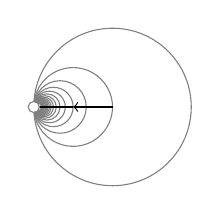
\begin{tikzpicture}
\foreach \i in {1,...,20}%
{%
	\draw[gray] ({1/\i},0) circle ({1/\i});
}%
\draw[->] (1,0) -- (.5,0);
\draw (.5,0) -- (0,0);
\fill[white,draw=gray] (0,0) circle (2pt);
\end{tikzpicture}
\end{center}

By the triangle inequality, if we head in any other direction, then \(r_{x(s)}\) goes up with at most unit speed.
So along any curve \(x(s)\) parameterized at unit speed,
\[
r_{x(0)}-s \le r_{x(s)} \le r_{x(0)}+s.
\]

Near enough to any point \(x_0\), \(r_x \ge r_{x_0}/2\), say in an open set.
Take any bump function \(f \ge 0\) so that, near \(x_0\), \(f(x) \ge 2/r_{x_0}\) and so that \(f=0\) outside some small neighborhood of \(x_0\).
Such open sets, equipped with bump functions, form an open cover.
Take a locally finite refinement, with associated bump functions \(f_i\).
Let \(f=\sum f_i\).
Then \(g' = f^2 g\) is a metric conformal to \(g\).

A compact curve parameterized as \(s \mapsto x(s)\) at unit \(g\)-speed with \(g\)-length \(\ell\) has \(g'\)-length
\[
\ell'=
\int f(x(s)) \, ds
\ge
\int \frac{ds}{r_{x(s)}}
\ge
\int \frac{ds}{s+r_{x_0}}
=
\log(1+\ell/r_{x_0}).
\]
If we fix a constant \(\varepsilon > 0\), then the compact \(g\)-ball of radius \((1-\varepsilon)r_{x_0}\) contains the \(g'\)-ball of radius \(\log(2-\varepsilon)\), hence both are compact.
If the compactness radius \(r'_{x_0}\) of \(g'\) is finite at a point \(x_0\), it decays as 
\[
r'_{x(s)}=r'_{x(0)}-s
\]
in some direction, so can't be always at least \(\log(2-\varepsilon)\).
Hence \(g'\) has infinite compactness radius.
By the Hopf--Rinow theorem, \(g'\) is complete.
\end{answer}


\section{Complex valued functions on the plane}
Every real analytic function on \(\C=\R[2]\), valued in the real or the complex numbers, has a unique convergent Taylor series
\[
f(x,y)= a_{00} + a_{10} x + a_{01} y + a_{20} \frac{x^2}{2} + a_{11}xy + a_{02} \frac{y^2}{2} + \dots.
\]
Write 
\begin{align*}
z &= x+iy, \\
\bar{z} &= x-iy,
\end{align*}
or equivalently,
\begin{align*}
x &= \frac{1}{2}(z+\bar{z}), \\
y &=\frac{i}{2}(\bar{z}-z).
\end{align*}
Plug in to the series expansion: every \emph{real analytic} complex-valued function \(f(x,y)\) has a unique convergent Taylor series expansion
\[
f(x,y)= b_{00} + b_{10} z + b_{01} \bar{z} + b_{20} \frac{z^2}{2} + b_{11}z\bar{z} + b_{02} \frac{\bar{z}^2}{2} + \dots.
\]
The function is holomorphic just when there are no \(\bar{z}\) terms.

Recall that \(\pderiv{x}{x}=1\) and \(\pderiv{y}{x}=0\).
It is convenient notation to introduce formal symbols \(\pdz{}\) and \(\pdzb{}\) so that
\(\pdz{z}=1\) and \(\pdz{\bar{z}}=0\), as if \(z\) and \(\bar{z}\) are independent variables.
(A physicist once apologized to me for doing this.)
More generally, they must differentiate formal Taylor series in \(z,\bar{z}\) as if \(z\) and \(\bar{z}\) were independent variables.
Check that the only possible operators that can solve such equations are
\begin{align*}
\pdz{}&\defeq\frac{1}{2}\pr{\pderiv{}{x}-i\pderiv{}{y}}, \\
\pdzb{}{}&\defeq\frac{1}{2}\pr{\pderiv{}{x}+i\pderiv{}{y}}.
\end{align*}

\section{The Beltrami equation}
Take any chart (maybe not conformal) defined near some point of \(M\), taking that point to the origin of the plane.
In that chart, say with coordinates \(z=x+iy\), \(\omega = a \, dz + b \, d\bar{z}\), say.
Make a linear change of variables to arrange that the coordinates \(z=x+iy\) are conformal at the origin.
So \(a=1\) and \(b=0\) at the origin.
So \(a\) is near \(1\) and \(b\) near \(0\) when we stay near the origin.
Let \(\mu=b/a\) and write \(\omega=a \, dz + b \, d\bar{z}=a(dz + \mu \, d\bar{z})\).
Any complex-valued function \(u\) has differential 
\begin{align*}
du 
&=
\pdz{u} dz + \pdzb{u} d\bar{z},
\\
&=
\pdz{u} (dz+\mu\,d\bar{z}) + \pr{ \pdzb{u} - \mu \pdz{u} } d\bar{z}.
\end{align*}
So \(u\) is conformal just when \(du\) is complex linear, just when
\[
\pdzb{u} = \mu \pdz{u},
\]
the \emph{Beltrami equation}.
The rank of this equation, as a pair of real linear equations in first derivatives, drops exactly when \(|\mu|=1\), as the reader can check.

A \emph{Beltrami equation}\define{Beltrami equation} is an equation
\[
\pdzb{u} = \mu \pdz{u},
\]
in the complex plane, written in the usual Euclidean derivatives, for some smooth complex-valued function \(\mu\) with \(|\mu|<1\).
If \(\mu\) is real analytic, the Beltrami equation is locally solvable by the Cauchy--Kovalevskaya\SubIndex{Cauchy--Kovalevskaya theorem}\SubIndex{theorem!Cauchy--Kovalevskaya} theorem.

Conversely, given any Beltrami equation in the complex plane, let
\[
\omega\defeq dz+\mu d\bar{z}.
\]
Then \(g=|\omega|^2\) is a Riemannian metric, with this Betrami equation as its equation of conformal maps, with orientation given by \(\omega_1,\omega_2\).

\begin{theorem}
Take an oriented surface \(M\) with a Riemannian metric \(g\).
Suppose that \(u\) is a conformal map from an open subset of \(M\) to an open subset of the plane, i.e. a holomorphic chart.
Then \(u\) satisfies the associated Beltrami equation.
Conversely, if \(u\) is a smooth complex valued solution of the associated Beltrami equation and \(du \ne 0\) at some point \(m_0 \in M\), then \(u\) is a conformal map of an open subset of \(M\) near \(m_0\), i.e. a holomorphic chart.
\end{theorem}
\begin{theorem}[The local uniformisation theorem (Korn--Lichtenstein) II]%
\define{theorem!Korn--Lichtenstein}\define{Korn--Lichtenstein theorem}
Every Beltrami equation has a local smooth solution \(u\), near any point \(m_0\), so that \(du\ne 0\) at \(m_0\). 
\end{theorem}
We will prove this theorem following \cite{Douady/Buff:2000}.
Since this theorem is local, in proving it, we can assume that \(\mu\) is smooth with compact support and \(|\mu|<1\) at every point of the complex plane.
Moreover, we can assume that \(\mu=0\) at any one chosen point.

\section{\texorpdfstring{\(L^2\) methods}{L2 methods}}
The \emph{Fourier transform}\define{Fourier transform} of an \(L^2\) function \(u\) on the plane \(\R[2]=\C\) is
\[
\hat{f}(\zeta)
=
\int_{\R[2]} f(x+iy) e^{-2 \pi i (x\xi + y \eta)}
\]
for \(\zeta = \xi + i \eta \in \C\); \cite{Folland:1992}. 
We recall that \(f \mapsto \hat{f}\) is an isomorphism of \(L^2\).

We easily check that, in the sense of distributions, 
\begin{align*}
\widehat{\pdz{f}} &= i \pi \zeta \hat{f}, \\
\widehat{\pdzb{f}} &= i \pi \bar\zeta \hat{f}.
\end{align*}
The \emph{Hilbert--Beurling operator}\define{Hilbert--Beurling operator} \(L\) is the operator so that
\[
\widehat{Lf}=(\bar\zeta/\zeta)\hat{f}.
\]
Since \(\zeta/\bar{\zeta}\) has norm 1 as a complex number, it doesn't alter \(L^2\) norms, so \(L\) is unitary.
Moreover, plugging in,
\[
L\pdz{} = \pdzb{}.
\]

\begin{theorem}
Take a smooth compact domain \(U \subset \C\).
To every \(f \in L^2(U)\), there is a unique \(u \in L^2(\C)\) so that 
\begin{enumerate}
\item \(\pdzb{u}=f\) and
\item both \(\pdz{u}\) and \(\pdzb{u}\) are also in \(L^2(\C)\).
\end{enumerate}
\end{theorem}
\begin{proof}
Recall the Cauchy\define{Cauchy integral theorem} integral theorem with remainder: if \(u\) is smooth on a smooth compact domain \(U \subset \C\):
\[
u(z) = \frac{1}{2 \pi i} \int_{\partial U} \frac{u(w) \, dw}{w-z} + \frac{1}{2 \pi i} \int_U \pdzb{u(w)}[w] \frac{dw \wedge d\bar{w}}{w-z}.
\]
The proof is just Stokes's theorem.

In particular, to solve the equation
\[
\pdzb{u} = f,
\]
in the complex plane, for any smooth compactly supported function \(f\), we can set
\[
u(z) = \frac{1}{2 \pi i} \int_{\C} f(w) \frac{dw \wedge d\bar{w}}{w-z}.
\]
Then \(u(z)=O(z^{-1})\) as \(z \to \infty\).
Also note that this is a convolution:
\[
u(z) = \frac{1}{\pi z} * f(z).
\]
The Hausdorff--Young\define{Hausdorff--Young inequality} inequality \cite{Lieb/Loss:2001} p. 98 theorem 4.2 says that if \(f\) is supported on some domain \(U \subset \C\) then
\[
\norm{u}[2] \le \norm{f}[2] \norm{\frac{1}{\pi z}}[1][U].
\]
So once we fix a compact domain \(U\) for \(f\) to be supported on, the map \(f \mapsto u\) is bounded and so extends to a linear map
\[
f \in L^2(U) \mapsto u \in L^2(\C).
\]
Moreover, since \(f\) has compact support, \(u\) is holomorphic outside of \(U\).
Note that
\[
\pdz{u} = L \pdzb{u} = Lf \in L^2(\C).
\]
\end{proof}

\begin{theorem}\label{theorem:L2}
Pick any smooth complex-valued function \(\mu \colon \C \to \C\) with compact support and with \(|\mu|<1\).
There is a unique solution \(u=u_{\mu}\) to the Beltrami equation 
\[
\pdzb{u} = \mu \pdz{u},
\]
of the form \(u(z)=z+\phi(z)\) where \(\phi \in L^2\) has \(L^2\) distributional derivatives.
\end{theorem}
\begin{proof}
The operator \(1-\mu L\) is bounded from below away from zero, so has an inverse on \(L^2\) given by geometric series
\[
(1-\mu L)^{-1}
=
1 + \mu L + (\mu L)^2 + \dots.
\]
Let \(f \defeq (1-\mu L)^{-1} \mu\).
Then \((1-\mu L)f = \mu\), i.e. \(f=\mu L f + \mu\).
Since \(\mu\) has compact support, say in some domain \(U \subset \C\), for any point outside of \(U\), this equation gives \(f=0\).
So \(f \in L^2(U)\).
Let \(\phi\) be the \(L^2\) function with 
\[
\pdzb{\phi}=f.
\]
Then plug into \(f=\mu L f + \mu\) to see that
\[
\pdzb{(z+\phi)}=\pdzb{\phi}=f=\mu L f + \mu = \mu \pdz{\phi} + \mu = \mu \pdz{(z+\phi)}.
\]
\end{proof}

\section{Smoothness}
So far, we have a solution \(u(z)=z + \phi(z)\) to the Beltrami equation, unique, with \(\phi,\pdz{\phi},\pdzb{\phi} \in L^2\).
We want to prove that \(u\) is smooth.
Since our problem is local, we can multiply \(\mu\) by a bump function, equal to 1 near 0 and to 0 not far away.
Since we have \(\mu(0)=0\), we can safely assume that \(\mu\) is uniformly as small as we like; we will suppose that \(|\mu|<1/3\).

\subsection{Distant peaks}
Take a continuous function \(y=h(x)\ge 0\) defined for \(x\ge 0\), with \(h(x) \to 0\) as \(x \to \infty\), but not rapidly, i.e. more slowly than some rational function.
Fix some positive integer \(k\).
Pick a positive integer \(n\). 
From among those \(x\) for which \(h(x) \ge n/x^k\), pick a point \(x=x_n\) at which \(h(x)\) is largest: call \(x_n\) a \emph{distant peak}.
As we make \(n\) larger, in any compact interval of values of \(x\), eventually we make \(n/x^k\) larger than \(h(x)\), so we have to find a more distant ``distant peak''.
By definition, \(x_n^k h(x_n) \ge n \to \infty\), so at distant peaks, \(h\) decays slowly, and, roughly speaking, nowhere more slowly.
\begin{center}
\documentclass{standalone}
\usepackage{pgfplots}
\begin{document}
\begin{tikzpicture}
	\begin{axis}[
		axis lines=none,
		domain=0:20,
		xtick style={draw=none},
		ytick style={draw=none},
		xticklabels={},
		yticklabels={},
	]
	% use TeX as calculator:
	\addplot[mark=none,blue,samples=150] {exp(-x/6)*sin(deg(x))};
	\addplot[mark=square] coordinates {(1.4,.78)};
	\addplot[mark=square] coordinates {(7.65,.27)};
	\addplot[mark=square] coordinates {(14,.095)};
	\end{axis}
\end{tikzpicture}
\end{document}

\end{center}
\begin{lemma}
Pick any function \(r \colon \R[> 0] \to \R[> 0]\) with \(r(x)=o(x)\) as \(x \to \infty\).
Write \(x\gtrsim x_n\) to mean \(x>x_n-r(x_n)\).

Take a continuous function \(h(x)\ge 0\) defined for \(x\ge 0\), with \(h(x) \to 0\) as \(x \to \infty\), but not rapidly.
For some integer \(k>0\), there are distant peaks \(x_n \to \infty\) where
\[
1 = \lim_{n \to \infty} \sup_{x\gtrsim x_n} \frac{h(x)}{h(x_n)}.
\]
\end{lemma}
\begin{proof}
If \(h(x) \ge n/x^k\), then \(h(x)\le h(x_n)\), by definition of a distant peak.
If \(h(x) < n/x^k\) then 
\[
h(x) < \frac{n}{x^k} = \frac{n}{x_n^k} \frac{x_n^k}{x^k} = h(x_n) \frac{x_n^k}{x^k}.
\]
If
\[
x \ge x_n-r(x_n),
\]
then
\[
\frac{x_n^k}{x^k} < \pr{\frac{x_n}{x_n-r(x_n)}}^k.
\]
So finally, for any \(x\) with \(x \ge x_n-r(x_n)\), 
\[
\frac{h(x)}{h(x_n)} \le \pr{\frac{x_n}{x_n-r(x_n)}}^k = \pr{\frac{1}{1-\frac{r(x_n)}{x_n}}}^k\to 1.
\]
\end{proof}

\subsection{Holding down the Fourier transform}
\begin{lemma}
Suppose that \(f \colon \C \to \C\) is continuous and \(f\) decays but not rapidly.
Roughly: we can find distant peaks \(\zeta_n\) of \(|f|\).
Precisely: pick any function \(r \colon \R[> 0] \to \R[> 0]\) with \(r(x)=o(x) \) as \(x \to \infty\).
Write \(x\gtrsim x_n\) if \(x>x_n-r(x_n)\).
For some integer \(k>0\), there are points \(\zeta_n \to \infty\) with \(|\zeta_n^k f(\zeta_n)| \to \infty\) and
\[
1 = \lim_{n \to \infty} \sup_{|\zeta|\gtrsim|\zeta_n|} \frac{|f(\zeta)|}{|f(\zeta_n)|}.
\]
\end{lemma}
\begin{proof}
Let 
\[
h(x) = \sup_{|\zeta|=x} |f(\zeta)|.
\]
\end{proof}

\begin{theorem}
Pick any smooth complex-valued function \(\mu \colon \C \to \C\) with compact support and with \(|\mu|<\frac{1}{3}\).
Then the solution \(u=u_{\mu}\) to the Beltrami equation 
\[
\pdzb{u} = \mu \pdz{u},
\]
defined in theorem~\vref{theorem:L2} is a smooth diffeomorphism.
\end{theorem}
\begin{proof}
Fourier transform the equation \(f=\mu L f + \mu\) to get
\[
\hat{f} = \hat{\mu} * (\bar\zeta/\zeta) \hat{f} + \hat\mu.
\]
Since \(\mu\) is smooth and compactly supported, it is Schwartz, so \(\hat\mu\) is Schwartz.
Convolution with \(\hat\mu\) is smoothing, so \(\hat{f}\) is smooth.
Take \(L^1\) norm:
\[
\norm{\hat{f}}[1] = \norm{\hat{\mu}}[1] \norm{\hat{f}}[1] + \norm{\hat{\mu}}[1],
\]
or
\[
\norm{\hat{f}}[1] 
= \frac{\norm{\hat{\mu}}[1]}{1-\norm{\hat{\mu}}[1]}
= \frac{\norm{\mu}[\infty]}{1-\norm{\mu}[\infty]}
< \frac{1}{2}.
\]
So 
\[
\norm{f}[\infty] \le \norm{\hat{f}}[1] < \frac{1}{2}.
\]
Hence
\[
\norm{\pdzb{\phi}}[\infty] < \frac{1}{2}.
\]
Note then that
\[
\norm{\pdz{\phi}}[\infty] = \norm{\widehat{\pdz{\phi}}}[1] =  \norm{(\bar\zeta/\zeta)\widehat{f}}[1] = \norm{\hat{f}}[1] < \frac{1}{2}.
\]
Hence writing \(u=z+\phi\), 
\[
\norm{\pdz{u}}[\infty] = \norm{1+\pdz{\phi}}[\infty] > \frac{1}{2}
\]
while
\[
\norm{\pdzb{u}}[\infty] = \norm{\pdz{\phi}}[\infty]  < \frac{1}{2}.
\]

It suffices to prove that \(f=\pdz{\phi}\) is smooth, so we can see that \(\phi\) is smooth from \(u=\frac{1}{\pi z} * f\).
To prove that \(f\) is smooth is to prove that \(\hat{f}\) decays even when multiplied by any polynomial function, i.e. decays rapidly, by the Plancherel theorem \cite{Folland:1995} p. 191 theorem 6.1.\SubIndex{Plancherel theorem}\SubIndex{theorem!Plancherel}
So suppose that \(\hat{f}\) fails to decay rapidly.

Apply the lemma above, we find the ``worst behaviour'' of \(\hat{f}\), i.e. the ``distant peaks'', occuring at some points \(\zeta_n\).
We can pick \(r \colon \R[>0] \to \R[>0]\) as long as \(r(x)/x \to 0\) as \(x \to \infty\) and, in addition, we add the assumption that \(r(x)\) is bounded below by some positive power of \(x\), as \(x \to \infty\).

Let
\[
\mu_n = 
\begin{cases}
\mu, & \text{ if \(|\zeta|<r(|\zeta_n|)\)}, \\
0, & \text{ otherwise}.
\end{cases}
\]
Note that since \(|\mu|<1/3\), we have \(|\mu_n|<1/3\), and so
\[
\norm{\hat\mu_n}[1]\le\norm{\hat\mu}[1]=\norm{\mu}[\infty]<\frac{1}{3}.
\]
The equation
\[
\hat{f} = \hat{\mu} * (\bar\zeta/\zeta) \hat{f} + \hat\mu
\]
tells us that
\[
\hat{f} = \hat{\mu}_n * (\bar\zeta/\zeta) \hat{f} + (\hat\mu-\hat{\mu}_n) * (\bar\zeta/\zeta) \hat{f} + \hat\mu,
\]
a sum of three terms.
The first term is convolved only inside a particular disk, so is at worst
\[
\left|
\hat{\mu}_n * (\bar\zeta/\zeta) \hat{f}
\right|
\le \frac{1}{3} \sup_{|\zeta-\zeta_n|\le r(|\zeta_n|)}|\hat{f}(\zeta)|.
\]
Plugging in our ``worst points'' \(\zeta=\zeta_n\):
\[
\left|
\hat{\mu}_n * (\bar\zeta/\zeta) \hat{f}
\right|
\le \frac{1}{3} |\hat{f}(\zeta_n)|(1+o(1)).
\]
The third term decays rapidly.
For the second term, 
\[
\norm{\hat\mu-\hat{\mu}_n}[1]
=\int_{|\zeta-\zeta_n|>r(|\zeta_n|)} |\hat\mu|
\] 
decays more rapidly than any power of \(|\zeta_n|\), as \(\hat\mu\) is Schwartz.
So finally,
\[
|\hat{f}(\zeta_n)| \le \frac{1}{3} |\hat{f}(\zeta_n)| (1+o(1)),
\]
which forces \(\hat{f}(\zeta_n) \to 0\), a contradiction to our hypothesis that \(\hat{f}\) does not decay rapidly.
\end{proof}
The Korn--Lichtenstein theorem follows.


\section{First order linear systems}
Take any system of two linearly independent first order partial differential equations,
\begin{align*}
0 &= a u_x + b u_y + c v_x + d v_y, \\
0 &= e u_x + f u_y + g v_x + h v_y
\end{align*}
with variable coefficients: \(a=a(x,y)\) and so on.
At any chosen point \((x,y)=(x_0,y_0)\), the differential
\[
\begin{pmatrix}
u_x & u_y \\
v_x & v_y
\end{pmatrix}
\]
of any solution belongs to a \(2\)-parameter family of linear maps cut out by our system.
\begin{problem}{kl:ellipticity}
Prove that the system is elliptic just when all determinants
\[
\det
\begin{pmatrix}
u_x & u_y \\
v_x & v_y
\end{pmatrix}
\]
of those nonzero linear maps satisfying our system are nonzero.
\end{problem}
\begin{problem}{kl:project}
Write that ellipticity condition in terms of the points
\[
\begin{bmatrix}
u_x\\
u_y\\
v_x\\
v_y
\end{bmatrix}
\]
in \(3\)-dimensional real projective space.
\end{problem}
\begin{answer}{kl:project}
At each point \((x_0,y_0)\), this 2-parameter family of linear maps projectivizes to a real projective line in 3-dimensional real projective space.
The differentials
\[
\begin{pmatrix}
u_x & u_y \\
v_x & v_y
\end{pmatrix}
\]
with determinant zero projectivize to a quadric surface in that projective space, a hyperboloid of one sheet.
If that line does not strike that hyperboloid at any real point, the system is elliptic.
\end{answer}
\begin{problem}{kl:rewrite.system}
Prove that, for any orientation of the \((x,y)\) plane, if we use one of these linear maps 
\[
\begin{pmatrix}
u_x & u_y \\
v_x & v_y
\end{pmatrix}
\]
to produce an orientation of the \((u,v)\) plane, then we can rewrite our system as a Beltrami equation.
\end{problem}
\begin{theorem}[The local uniformisation theorem III (Korn--Lichtenstein)]
Every smooth linear elliptic system of 2 first order equations for 2 functions of 2 variables has a local smooth solution \((u,v)\), near any point \((x_0,y_0)\), so that 
\[
0 \ne 
\det
\begin{pmatrix}
u_x & u_y \\
v_x & v_y
\end{pmatrix}(x_0,y_0).
\]
After the change of variables replacing \((x,y)\) by any one such solution \((u,v)\), the system becomes the Cauchy--Riemann equations.
\end{theorem}
\begin{problem}{kl:solve.2nd.order}
Prove the local solvability of any 2nd order elliptic partial differential equation of the form
\[
0=au_{xx}+bu_{xy}+cu_{yy}+du_x+eu_y.
\]
\end{problem}
